\section{实验分析和总结}
    \subsection{数据结构分析}
        \par 由于文本编辑器需要实现频繁的插入、删除操作,所以我选择了链串+链表的实现方法,从整体上来看,这个数据结构很好地实现实验所提出的各项要求,但仍有不足:
        \begin{itemize}
            \item 链串在应对大规模数据时的运行效率十分低下,只能处理较轻量的文本
            \item 由于链串的内存区域并不连续,不能善加利用缓存,导致在遍历时的运行时间要远大于其他数据结构
        \end{itemize}
    \subsection{算法复杂度分析}
        \par 在代码解释时说明了各函数的时间复杂度,故此处只对其进行汇总
        \begin{itemize}
            \item 操作一:根据之前的分析,时间复杂度为 \textbf{O(nm)}
            \begin{figure*}[htbp]
                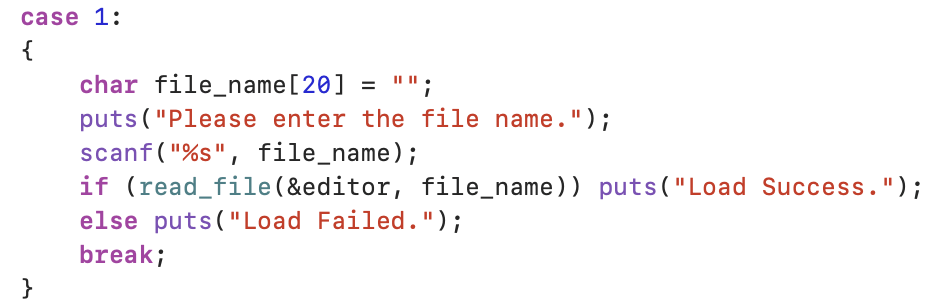
\includegraphics[width = 10cm]{cs_1.png}
            \end{figure*}
            \item 操作二:根据之前的分析,时间复杂度为 \textbf{O(nm)}
            \begin{figure*}[htbp]
                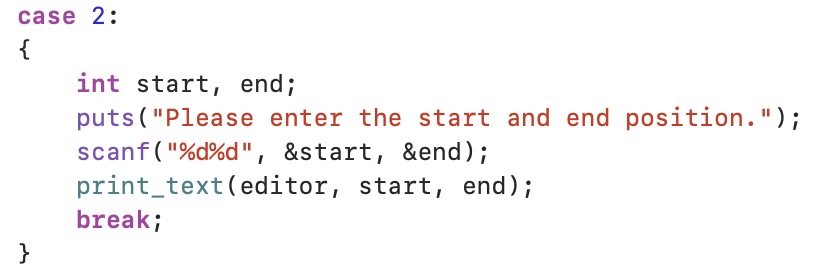
\includegraphics[width = 10cm]{cs_2.png}
            \end{figure*}
            \newpage
            \item 操作三:根据之前的分析,时间复杂度为 \textbf{O(n + m)}
            \begin{figure*}[htbp]
                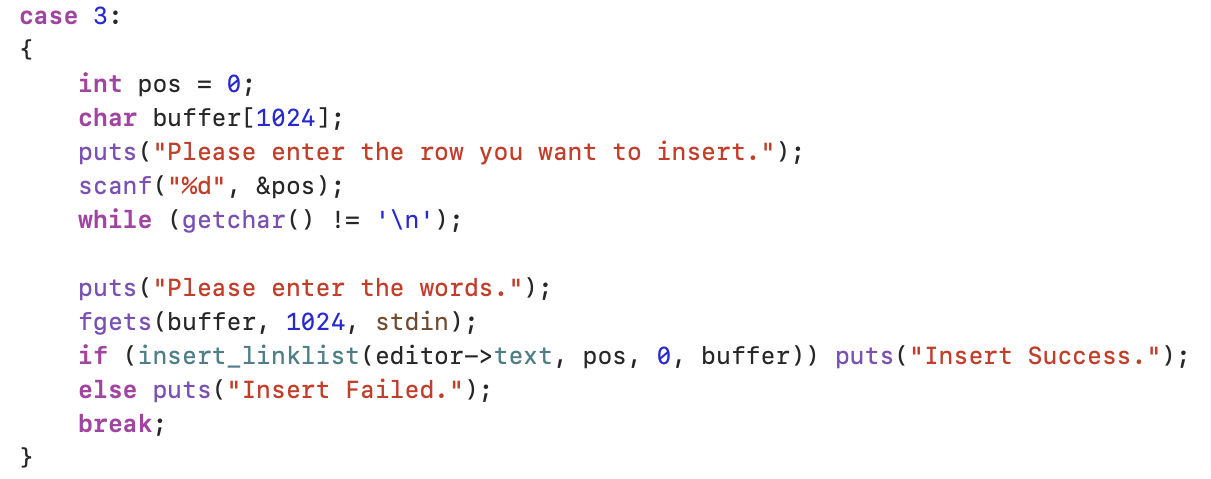
\includegraphics[width = 12cm]{cs_3.png}
            \end{figure*}
            \item 操作四:根据之前的分析,时间复杂度为 \textbf{O(n + m)}
            \begin{figure*}[htbp]
                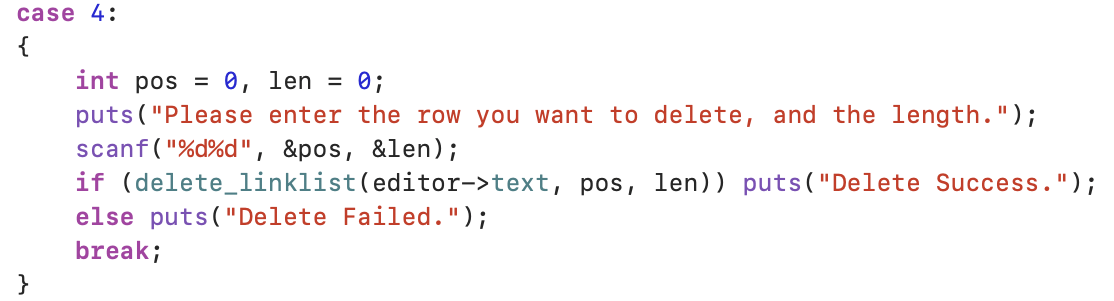
\includegraphics[width = 12cm]{cs_4.png}
            \end{figure*}
            \item 操作五:根据之前的分析,时间复杂度为 \textbf{O(n + m)}
            \begin{figure*}[htbp]
                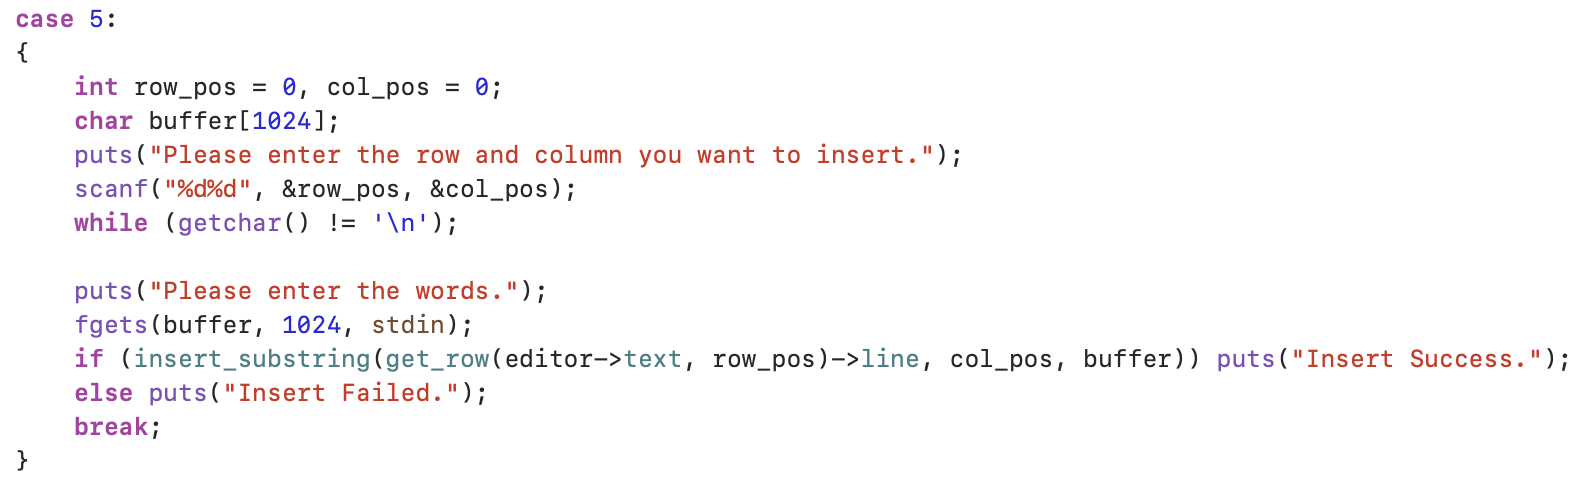
\includegraphics[width = 16cm]{cs_5.png}
            \end{figure*}
            \newpage
            \item 操作六:根据之前的分析,时间复杂度为 \textbf{O(n + m)}
            \begin{figure*}[htbp]
                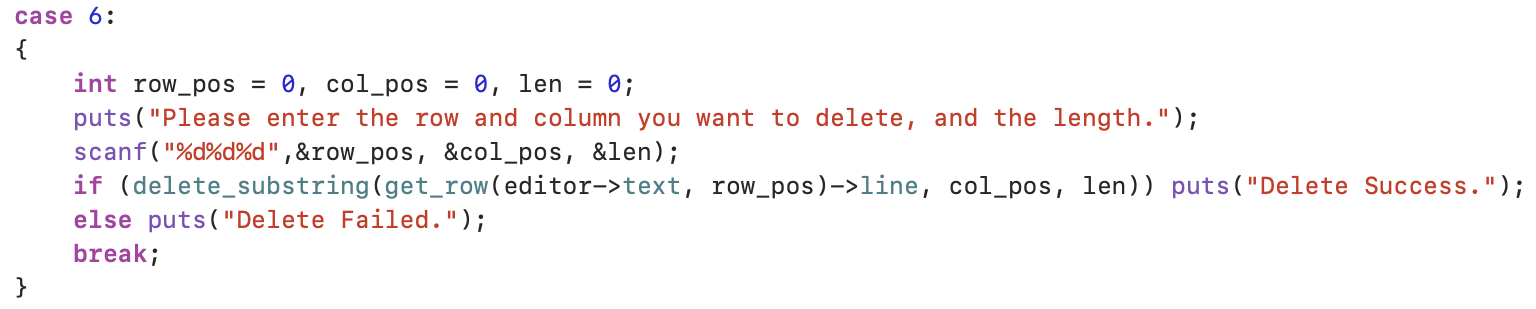
\includegraphics[width = 15cm]{cs_6.png}
            \end{figure*}
            \item 操作七:根据之前的分析,时间复杂度为 \textbf{O(n + m)}
            \begin{figure*}[htbp]
                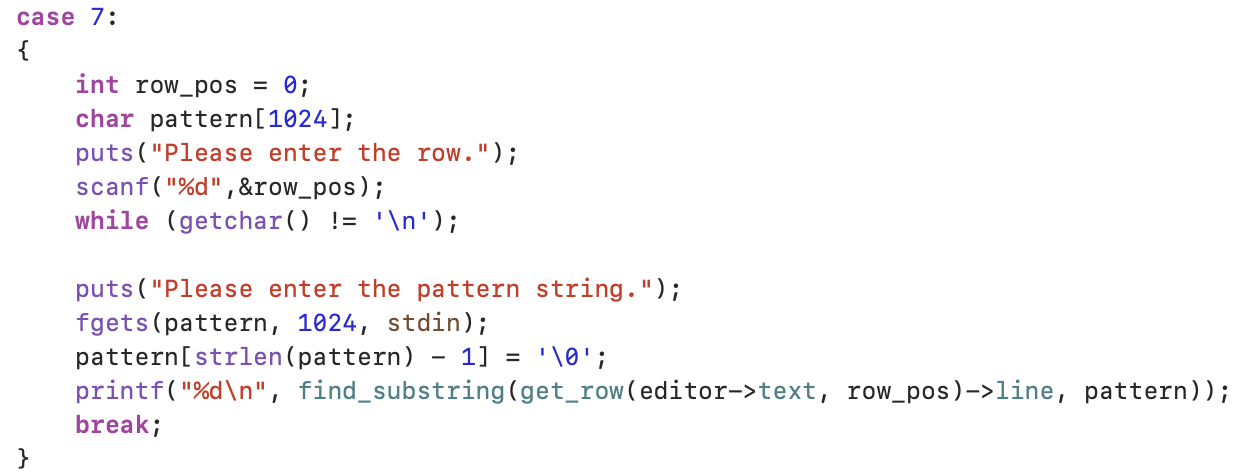
\includegraphics[width = 14cm]{cs_7.png}
            \end{figure*}
            \item 操作八:根据之前的分析,时间复杂度为 \textbf{O(nm)}
            \begin{figure*}[htbp]
                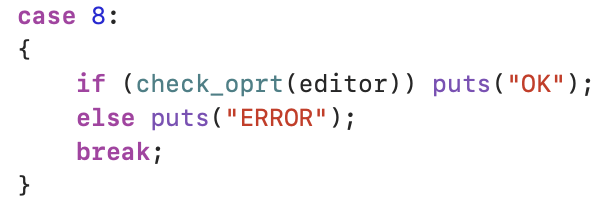
\includegraphics[width = 8cm]{cs_8.png}
            \end{figure*}
            \newpage
            \item 操作九:根据之前的分析,时间复杂度为 \textbf{O(nm)}
            \begin{figure*}[htbp]
                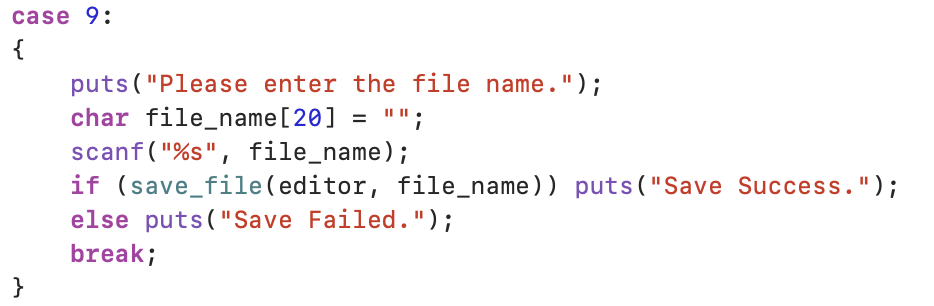
\includegraphics[width = 10cm]{cs_9.png}
            \end{figure*}
        \end{itemize}
    \subsection{总结}
        \par 通过这次实验,我学习了如何编写和使用链表、链串和栈来解决实际问题;在输入数据时,考虑到 \textbf{scanf(``\%s")} 不能读取空格,我使用了 \textbf{fgets()} 函数,但在读入时程序总会崩溃。通过查阅资料,我了解了缓冲区及相关概念,并解决了该问题。但这次实验仍有很多小问题,比如代码不够简洁,代码的复用性不强等,导致最后整体代码量比较大。
